\chapter{Kết quả và thảo luận}
\label{ch:ketquaphantich}

\section{Các phương pháp phân tích số liệu}

Trình bày phương pháp phân tích số liệu. 

Có thể đưa các đoạn văn bản, công thức toán học, hình vẽ, bảng biểu, v.v., vào đây. Có thể bổ sung thêm các mục hoặc các tiểu mục khác thông qua lệnh section, subsection hay subsubsection v.v.

\section{Các kết quả chính}

\begin{figure}[!htb]
\centering
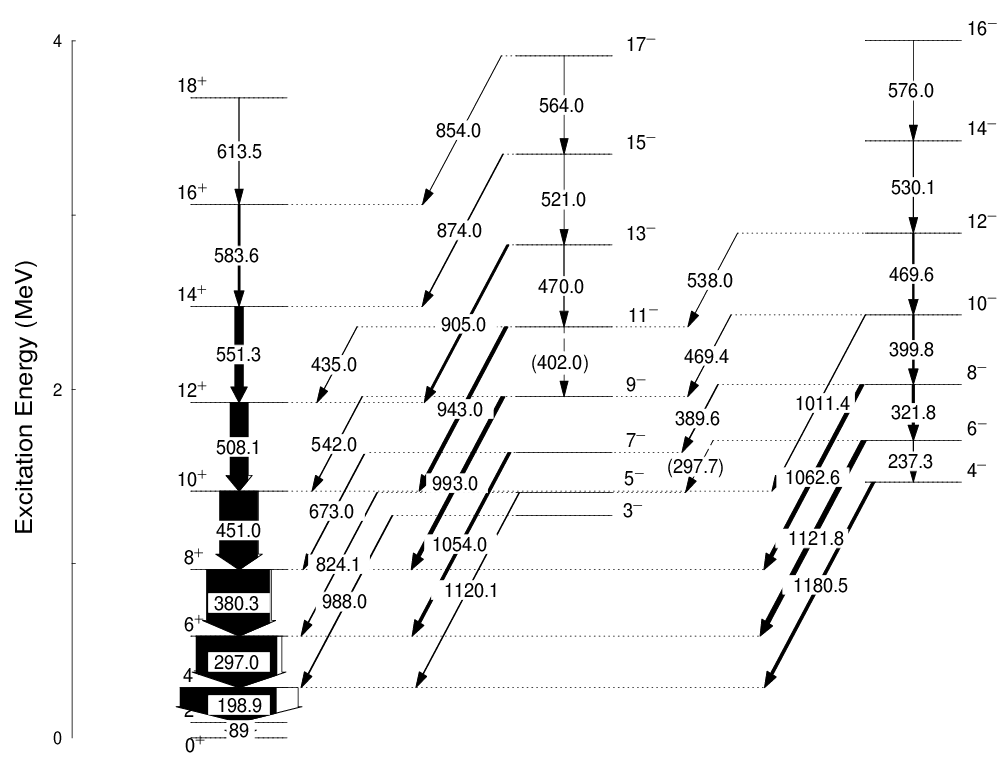
\includegraphics[width=0.4\textwidth]{figure/fig_ketquaphantich/156Gd.png}
\caption{Các mức năng lượng và tỷ lệ các chuyển dịch giữa các mức năng lượng của hạt nhân 156Gd được xác định bằng thực nghiệm.}
\label{fig:156Gd}
\end{figure} 

Trình bày các kết quả. 

Có thể đưa các đoạn văn bản, công thức toán học, hình vẽ, bảng biểu, v.v., vào đây. Có thể bổ sung thêm các mục hoặc các tiểu mục khác thông qua lệnh section, subsection hay subsubsection v.v.

Các mức năng lượng của hạt nhân 156Gd được thể hiện trên Hình \ref{fig:156Gd}.